% -*- program: xelatex -*-

%%%%%%%%%%%%%%%%%%%%%%%%%%%%%%%%%%%%%%%%%
% Wilson Resume/CV
% XeLaTeX Template
% Version 1.0 (22/1/2015)
%
% This template has been downloaded from:
% http://www.LaTeXTemplates.com
%
% Original author:
% Howard Wilson (https://github.com/watsonbox/cv_template_2004) with
% extensive modifications by Vel (vel@latextemplates.com)
%
% License:
% CC BY-NC-SA 3.0 (http://creativecommons.org/licenses/by-nc-sa/3.0/)
%
%%%%%%%%%%%%%%%%%%%%%%%%%%%%%%%%%%%%%%%%%

%----------------------------------------------------------------------------------------
%	PACKAGES AND OTHER DOCUMENT CONFIGURATIONS
%----------------------------------------------------------------------------------------

\documentclass[10pt]{article} % Default font size
\usepackage{graphicx}

%%%%%%%%%%%%%%%%%%%%%%%%%%%%%%%%%%%%%%%%%
% Wilson Resume/CV
% Structure Specification File
% Version 1.0 (22/1/2015)
%
% This file has been downloaded from:
% http://www.LaTeXTemplates.com
%
% License:
% CC BY-NC-SA 3.0 (http://creativecommons.org/licenses/by-nc-sa/3.0/)
%
%%%%%%%%%%%%%%%%%%%%%%%%%%%%%%%%%%%%%%%%%

%----------------------------------------------------------------------------------------
%	PACKAGES AND OTHER DOCUMENT CONFIGURATIONS
%----------------------------------------------------------------------------------------

\usepackage[a4paper, hmargin=25mm, vmargin=30mm, top=20mm]{geometry} % Use A4 paper and set margins

\usepackage{fancyhdr} % Customize the header and footer

\usepackage{lastpage} % Required for calculating the number of pages in the document

\usepackage{hyperref} % Colors for links, text and headings

\setcounter{secnumdepth}{0} % Suppress section numbering

%\usepackage[proportional,scaled=1.064]{erewhon} % Use the Erewhon font
%\usepackage[erewhon,vvarbb,bigdelims]{newtxmath} % Use the Erewhon font
\usepackage[utf8]{inputenc} % Required for inputting international characters
\usepackage[T1]{fontenc} % Output font encoding for international characters

\usepackage{fontspec} % Required for specification of custom fonts
\setmainfont[Path = ./fonts/,
Extension = .otf,
BoldFont = Erewhon-Bold,
ItalicFont = Erewhon-Italic,
BoldItalicFont = Erewhon-BoldItalic,
SmallCapsFeatures = {Letters = SmallCaps}
]{Erewhon-Regular}

\usepackage{color} % Required for custom colors
\definecolor{slateblue}{rgb}{0.17,0.22,0.34}

\usepackage{sectsty} % Allows customization of titles
\sectionfont{\color{slateblue}} % Color section titles

\fancypagestyle{plain}{\fancyhf{}\cfoot{\thepage\ of \pageref{LastPage}}} % Define a custom page style
\pagestyle{plain} % Use the custom page style through the document
\renewcommand{\headrulewidth}{0pt} % Disable the default header rule
\renewcommand{\footrulewidth}{0pt} % Disable the default footer rule

\setlength\parindent{0pt} % Stop paragraph indentation

% Non-indenting itemize
\newenvironment{itemize-noindent}
{\setlength{\leftmargini}{0em}\begin{itemize}}
{\end{itemize}}

% Text width for tabbing environments
\newlength{\smallertextwidth}
\setlength{\smallertextwidth}{\textwidth}
\addtolength{\smallertextwidth}{-2cm}

\newcommand{\sqbullet}{~\vrule height 1ex width .8ex depth -.2ex} % Custom square bullet point definition

%----------------------------------------------------------------------------------------
%	MAIN HEADER COMMAND
%----------------------------------------------------------------------------------------

\renewcommand{\title}[1]{
{\huge{\color{slateblue}\textbf{#1}}}\\ % Header section name and color
\rule{\textwidth}{0.5mm}\\ % Rule under the header
}

%----------------------------------------------------------------------------------------
%	JOB COMMAND
%----------------------------------------------------------------------------------------

\newcommand{\job}[6]{
\begin{tabbing}
\hspace{2cm} \= \kill
\textbf{#1} \> \href{#4}{#3} \\
\textbf{#2} \>\+ \textit{#5} \\
\begin{minipage}{\smallertextwidth}
\vspace{2mm}
#6
\end{minipage}
\end{tabbing}
\vspace{2mm}
}

%----------------------------------------------------------------------------------------
%	SKILL GROUP COMMAND
%----------------------------------------------------------------------------------------

\newcommand{\skillgroup}[2]{
\begin{tabbing}
\hspace{5mm} \= \kill
\sqbullet \>\+ \textbf{#1} \\
\begin{minipage}{\smallertextwidth}
\vspace{2mm}
#2
\end{minipage}
\end{tabbing}
}

%----------------------------------------------------------------------------------------
%	INTERESTS GROUP COMMAND
%-----------------------------------------------------------------------------------------

\newcommand{\interestsgroup}[1]{
\begin{tabbing}
\hspace{5mm} \= \kill
#1
\end{tabbing}
\vspace{-10mm}
}

\newcommand{\interest}[1]{\sqbullet \> \textbf{#1}\\[3pt]} % Define a custom command for individual interests

%----------------------------------------------------------------------------------------
%	TABBED BLOCK COMMAND
%----------------------------------------------------------------------------------------

\newcommand{\tabbedblock}[1]{
\begin{tabbing}
\hspace{2cm} \= \hspace{4cm} \= \kill
#1
\end{tabbing}
} % Include the file specifying document layout
\hfuzz=20pt
\vfuzz=29pt
\hbadness=20000
\vbadness=\maxdimen

%----------------------------------------------------------------------------------------

\begin{document}

%----------------------------------------------------------------------------------------
%	NAME AND CONTACT INFORMATION
%----------------------------------------------------------------------------------------

\title{Mark Arts -- Resume} % Print the main header

%------------------------------------------------

\parbox{0.5\textwidth}{ % First block
\begin{tabbing} % Enables tabbing
\hspace{3cm} \= \hspace{4cm} \= \kill % Spacing within the block
{\bf Date of Birth} \> 6$^{th}$ April 1993 \\ % Date of birth
{\bf Nationality} \> Dutch \\% Nationality
{\bf Email} \> \href{mailto:marktarts93@gmail.com}{marktarts93@gmail.com} \\ % Email address
\end{tabbing}}

%----------------------------------------------------------------------------------------
%	PERSONAL PROFILE
%----------------------------------------------------------------------------------------

\begin{figure}[ht]
  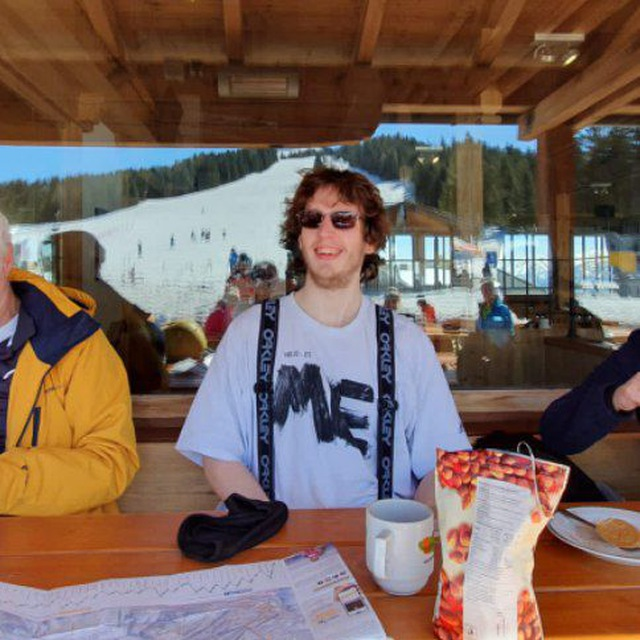
\includegraphics[width=0.33\linewidth]{1.jpg}
  
\includegraphics[width=0.33\linewidth]{2.jpg}
  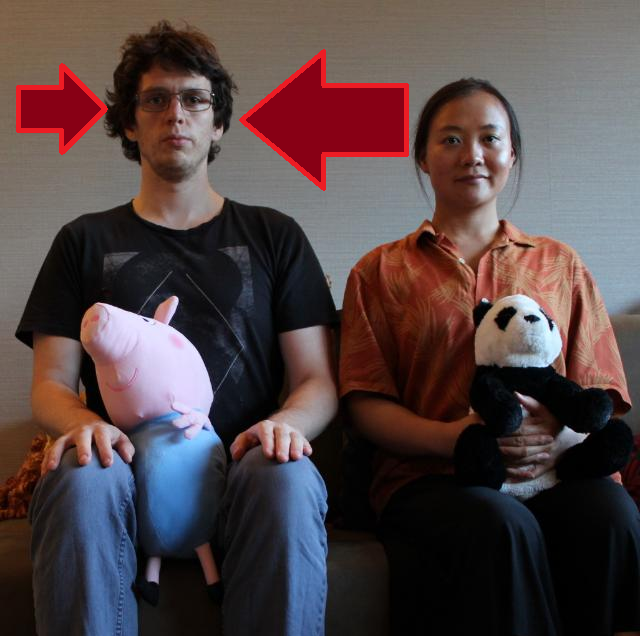
\includegraphics[width=0.33\linewidth]{3.png}
\end{figure}

\section{Personal Profile}

I'm a passionate and curious programmer with a broad skill set looking for a position where he can utilize and learn interesting technologies and tools. \\

I started programming for my bachelor and quickly decided to combine my studies with work to learn what it means to work in a professional context. After finishing my studies, I worked as a backender and later DevOps, in which roles I actively engaged with the technologies around me, making sure to pick up tasks outside my skillset to expand my knowledge and experience, for example, picking up FE stories from the backlog. \\

My more recent focus has been on developing my soft skills as a team lead, providing my teammates opportunities to develop their skills, improving our processes by regular reflection, taking charge of our infrastructure efficiency, security, cost, and reliability, and transforming business requirements into actionable stories.

Besides web development and DevOps, I enjoy reading and learning about Artificial Intelligence, security/hacking, game development, mental and physical health, Blockchains, and most subjects regularly discussed on Hacker News. \\

One of my biggest hobbies is music. It's the perfect outlet for my curiosity, creativity, drive to improve, and playfulness. All aspects of music are interesting to me, from songwriting to physically playing instruments to mastering songs and everything in between. Giving me an endless playground for self-improvement and learning.  \\

I'm a fast and enthusiastic learner that is always up for a new challenge.

%----------------------------------------------------------------------------------------
%	EDUCATION SECTION
%----------------------------------------------------------------------------------------

\section{Education}

\tabbedblock{
  \bf{2010-2017} \> BSc in Media Technology - \href{https://www.rotterdamuas.com}{Rotterdam University of Applied Sciences} \\[5pt]
  \>Minor in Game Design and Development \\[5pt]
  \>Thesis: How can we realize a digital environment in which non-programmers, like 3D \\ \> modelers and level designers, can build an efficient and unique Virtual Reality experience
}

%------------------------------------------------

\tabbedblock{
  \bf{2005-2010} \> Higher General Secondary Education - Emmauscollege, Rotterdam\\[5pt]
}

%----------------------------------------------------------------------------------------
%	EMPLOYMENT HISTORY SECTION
%----------------------------------------------------------------------------------------

\section{Employment History}

\job
{May 2017 -}{Now}
{GUTS / GET-protocol, Amsterdam, Netherlands}
{http://guts.tickets}
{DevOps / Developer}
{As the first DevOps engineer at GUTS, I was responsible for the creation and maintenance of the infrastructure of the GUTS ticketing system, which grew from a single Django service to a microservice architecture running on K8s hosted on AWS K8s, implementing modern practices like ArgoCD deployment management, Hub-Spoke private networking, role-based short-lived access tokens through SSO and more. My tasks also included creating and maintaining our internal tooling, including GitLab, GitHub, CI (continuous integration/testing), metric/log aggregation and visualization, error reporting, backups, security, performance, and others. I also took ownership over improving knowledge sharing and code quality across all our disciplines through retros, workshops, hack days, lightning talks, and other activities. Next to my DevOps responsibilties I worked as both Backend and Frontend developer. During my time at GUTS I grew from a junior DevOps to a full-fledged team lead with full responsibility over a modern infrastructure stack.

\rule{0mm}{5mm}\textbf{Technologies:} Linux, Python, Go (Golang), Typescript, Ansible, Terraform, Argocd, Pulumi, Django, Flask, Deno, Docker, Nix, Vue, AWS, Azure, ELK, Grafana, GitLab, Github, Newrelic, Prometheus, Sentry, CI}

\job
{Aug 2016 -}{May 2017}
{Hoppinger, Rotterdam, Netherlands}
{http://www.hoppinger.com}
{DevOps / Developer}
{After my graduation internship, I returned to working at Hoppinger while finishing my study. In this year, I started focusing more on building automation for DevOps and server management through Puppet.

\rule{0mm}{5mm}\textbf{Technologies:} Puppet, Bash, PHP, Ruby, Rails, WordPress, Nix, Docker, Gulp, Linux, Apache, NGINX }

\job
{Feb 2016 -}{Jun 2016}
{DPI, Den Haag, Netherlands}
{http://www.dpi.com}
{Graduation Internship}
{I researched the possibility for 3D studios to create interactive VR stories without the need for a programmer in the Unreal Engine utilizing its visual scripting system Blueprints.\\

\rule{0mm}{5mm}\textbf{Technologies:} Unreal Engine 4, Blueprints, C++, Virtual Reality}

\job
{Feb 2013 -}{Feb 2016}
{Hoppinger, Rotterdam, Netherlands}
{http://www.hoppinger.com}
{Internship / working student}
{After my internship at Hoppinger I stayed to reinforce the service and support team. As a service and support member I was responsible for the maintenance and small feature requests for Wordpress, Rails and Drupal projects. When I was available full-time, for example vacations, I worked on building bigger projects.

\rule{0mm}{5mm}\textbf{Technologies:} PHP, Ruby, Javascript, Sass, Less, Python, Erb, Haml, Wordpress. Ruby on Rails, NodeJS, Puppet, Drupal, Gulp, Drush, Composer, NGINX, Apache, Git, Polymer, React, MySQL, PostgreSQL, Elasticsearch
}

\job
{Jul 2012 -}{Aug 2012}
{Unitas, Rotterdam, Netherlands}
{http://www.unitas.nl}
{Junior Developer}
{In the summer after the second year of my bachelor I worked for a company that created a software package to submit import and export request to the dutch customs.

\rule{0mm}{5mm}\textbf{Technologies:} WinDev, EDIFACT
}

%----------------------------------------------------------------------------------------
%	IT/COMPUTING SKILLS SECTION
%----------------------------------------------------------------------------------------

\section{Software Engineering Skills}

%------------------------------------------------

\skillgroup{Operations}
{
\textit{Ansible}\\
\textit{Terraform}\\
\textit{Pulumi}\\
\textit{Docker}\\
\textit{Nix(os)}\\
\textit{k8s}\\
\textit{sops}\\
\textit{Argocd}\\
\textit{Newrelic}\\
\textit{Grafana}\\
\textit{Kibana}\\
\textit{Cloudwatch}\\
\textit{Lambda}\\
\textit{EC2}\\
\textit{Cloudfront}\\
\textit{Cloudflare}\\
\textit{Netlify}\\
\textit{Stackpath}\\
\textit{Hub-Spoke networking with transit gateways}\\
\textit{Wireguard}\\
\textit{Google admin}\\
}

\skillgroup{State management} {
\textit{Couchdb}\\
\textit{Postgress}\\
\textit{Rabbitmq}\\
\textit{Redis}\\
\textit{Elasticache}\\
\textit{DynamoDB}\\
\textit{Prometheus}\\
\textit{Elasticsearch}\\
\textit{S3}\\
}

\skillgroup{Programming Languages in production}
{
\textit{Python}\\
\textit{Go}\\
\textit{Ruby}\\
\textit{HSL (Terraform)}\\
\textit{PHP}\\
\textit{C++}\\
\textit{C\#}\\
\textit{Javascript}\\
\textit{Typescript}\\
\textit{Bash/sh} - Server scripting / automation
}

\skillgroup{Programming Languages in hobby projects}
{
  \textit{Elixer}\\
  \textit{Haskell}\\
  \textit{Java}\\
  \textit{Lisp}\\
  \textit{Lua} \\
  \textit{Clojure}\\
}

%------------------------------------------------

\skillgroup{Web Development}
{
\textit{Vue, react-native}\\
\textit{GO, Django, Flask, Ruby on Rails, Wordpress, Drupal}\\
}

%----------------------------------------------------------------------------------------
%	INTERESTS SECTION
%----------------------------------------------------------------------------------------

\section{Interests}

\interestsgroup{
 \interest{Running, Cycling, Yoga, Weight lifting, Cooking, Mental and physical health}
 \interest{Music, Composing, Producing, Sound design, Piano, Accordion, Guitar, Modular Synthesizers}
 \interest{AI, Security, Game development, Blockchain, Hacking, Hacker News}
}

\end{document}
